\documentclass[UTF8]{ctexart}
\usepackage{amsmath}
\usepackage{amssymb}
\usepackage{background}
\usepackage{booktabs}
\usepackage{caption,subcaption}
\usepackage{enumitem}
\usepackage{float}
\usepackage{fontspec}
\usepackage{geometry}
\usepackage{makecell}
\usepackage{mathptmx} %mathptmx和times结合使得公式使用times new roman字体
\usepackage{pifont}
\usepackage{tasks}
\usepackage{tcolorbox}
\tcbuselibrary{breakable, raster}
\usepackage{tikz}
\usetikzlibrary{arrows.meta}
\usepackage{times}
\usepackage{xcolor}

\geometry{a5paper, top=0.1cm, left=1cm, right=1cm, bottom=1cm, footskip=0.6cm, marginparsep=0.1cm}

\setCJKmainfont[BoldFont={汉仪文黑-85W},ItalicFont={方正苏新诗柳楷简体}]{汉仪文黑-55W}
\setfontfamily\Issue{Century Schoolbook}
\setfontfamily\Genshin{Genshin Teyvat Lingua Franca}
\newfontfamily\timesnewroman{Times New Roman}
\setmainfont{Times New Roman}
\newCJKfontfamily\TitleFont{思源宋体 CN Heavy}
\captionsetup{font=small, labelfont=bf}
\setlist[itemize]{itemsep=0pt, parsep=0pt}
%\reversemarginpar

%\CTEXsetup[format = {\centering\bfseries\large}, beforeskip = 3pt, afterskip = 3pt]{section}
\CTEXsetup[format = {\color{cyan!50!black}\bfseries\large}]{subsection}
\settasks{label={\Alph*.}, label-format={\color{cyan!50!black}}, item-format={\color{cyan!50!black}},}

\newtcolorbox{mybox}{colback=cyan!10, colframe=cyan!50!black, boxrule=0.5pt, breakable}

\colorlet{darkcyan}{cyan!50!black}
\newcommand\Black[1]{\textcolor[gray]{0.3}{#1}}
\newcommand\Brown[1]{\textcolor[HTML]{998A4E}{#1}}
\newcommand\Emph[1]{\colorbox{green!10}{\textcolor{green!30!black}{\textbf{#1}}}}
\newcommand\Concept[1]{\textcolor{cyan!70!black}{#1}}
\newcommand\Notes[1]{\textcolor{yellow!50!black}{\small #1}}
\newcommand\Example[1]{\textcolor{cyan!70!black}{\small #1}}
\newcommand\means[1]{\textcolor{cyan!70!black}{#1}}

\newcommand\Ohm{\text{\timesnewroman Ω}}

\newcommand\IssueNumber{27}
\newcommand\Date{2024-5-15}
%\newcommand\Contributer{@金光日}
\newcommand\Subject{数据结构与算法}
\newcommand\Source{2023 考研 408 第 9 题}


\begin{document}
\backgroundsetup{contents=\includegraphics{上半示例.png}, center, scale=1, angle=0, opacity=1}
\BgThispage
\begin{center}
%{\scriptsize\Issue \textcolor[HTML]{C8BA83}{\Genshin WEEKLY TIPS}}
\phantom{...}

{\Large\textcolor{brown!40!white}{\makebox[10cm][s]{\Genshin WEEKLY KNOWLEDGE TIPS}}}

\vspace{-2em}

{\Huge\bfseries\TitleFont \Black{知\ 识\ 小\ 料}}


\vspace{-0.1cm}
{\footnotesize \Brown{「电计 2203 班」周常规知识整理共享}}
\end{center}

\vspace{-0.5cm}


\begin{figure}[H]
\hspace{1cm}
\begin{minipage}[t]{0.3\textwidth}
\centering
    \Brown{\Genshin ISSUE}

    \vspace{-0.6cm}
    \Huge \Issue\slshape\bfseries\Black{\IssueNumber}
\end{minipage}
\hfill
\begin{minipage}[t]{0.35\textwidth}
\small
\centering
    \Brown{日期:\Date} \\
%\vspace{-0.1cm}
%    \Brown{贡献者:\Contributer} \\
\vspace{-0.1cm}
    \Brown{学科:\Subject} \\
\vspace{-0.1cm}
    \Brown{来源:\Source}
\end{minipage}
\hspace{0.8cm}
\end{figure}

{\color{cyan!50!black}
现有长度为 5,初始为空的散列表 $HT$,散列函数 $H(k) = (k+4)\mod 5$,用线性探查再散列法解决冲突。若将关键字序列 2022, 12, 25 依次插入 $HT$ 中,然后删除关键字 25,则 $HT$ 中查找失败的平均查找长度为
\begin{tasks}(4)
    \task 1
    \task 1.6
    \task 1.8
    \task 2.2
\end{tasks}
}

模拟插入和删除流程:
\begin{itemize}[itemsep=0pt]
  \item 插入 2022,映射 $H(2022)=1$,位置空闲,直接插入位置 $h=1$ 
  \item 插入 12,映射 $H(12)=1$,位置被占用,线性探测插入位置 $h=1+1=2$
  \item 插入 25,映射 $H(25)=4$,位置空闲,直接插入位置 $h=4$
  \item 删除 25,映射 $H(25)=4$,将此处标记为「已删除」(\Emph{查找时记为非空闲})
\end{itemize}

\begin{figure}[htb]
  \centering
  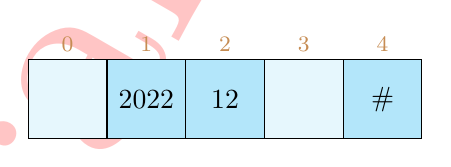
\begin{tikzpicture}
    \filldraw[fill=cyan!10] (0,0) rectangle (1,1);
    \filldraw[fill=cyan!30] (1,0) rectangle (2,1) node[midway] {2022};
    \filldraw[fill=cyan!30] (2,0) rectangle (3,1) node[midway] {12};
    \filldraw[fill=cyan!10] (3,0) rectangle (4,1);
    \filldraw[fill=cyan!30] (4,0) rectangle (5,1) node[midway] {\#};
    \foreach \i in {0,1,2,3,4}
        \node[font=\footnotesize, color=brown!90!] at (\i+0.5, 1.2) {\i};
  \end{tikzpicture}
\end{figure}

接下来模拟查找流程:设查找数映射的值为 $h$,因为是线性探查再散列,所以查找位置序列为:$h \to (h+1)\to (h+2)\to \cdots$。由于要求\Emph{「查找失败」}的次数,因此必定不会成功(表中的数必定不会等于查找数),依次查找直到遇到\Emph{「空闲」}的位置就停下即可。

\begin{itemize}[itemsep=0pt,parsep=0pt]
  \item 假如 $h=0$,则查找次数为 1;
  \item 假如 $h=1$,则查找次数为 3(挪到 $h=1\to 2\to 3$ 才空闲);
  \item 假如 $h=2$,则查找次数为 2(挪到 $h=2\to 3$ 才空闲);
  \item 假如 $h=3$,则查找次数为 1;
  \item 假如 $h=4$,则查找次数为 2(挪到 $h=4\to 0$ 才空闲)。
\end{itemize}

对上述 5 种可能的情况作出加权平均即可:

\begin{equation*}
   ASL_{\text{失败}} = \dfrac{1+3+2+1+2}{5} = 1.8
\end{equation*}

\newpage
\backgroundsetup{contents=\includegraphics{下半示例.png}, center, scale=1, angle=0, opacity=1}
\BgThispage

这个题到此已经做出来了。不过接下来可以简单讲一下为什么删除元素要将格子标记为「已删除」而非直接删除。

比如这回散列表长度为 5,$H(k)=k\mod 5$,线性探查再散列避免冲突。先后插入 3 和 8,得到的散列表肯定是这样的:

\begin{figure}[htb]
  \centering
  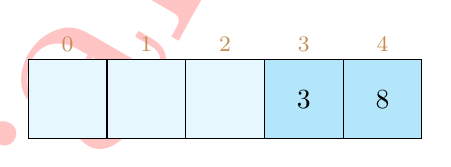
\begin{tikzpicture}
    \filldraw[fill=cyan!10] (0,0) rectangle (1,1);
    \filldraw[fill=cyan!10] (1,0) rectangle (2,1);
    \filldraw[fill=cyan!10] (2,0) rectangle (3,1);
    \filldraw[fill=cyan!30] (3,0) rectangle (4,1) node[midway] {3};
    \filldraw[fill=cyan!30] (4,0) rectangle (5,1) node[midway] {8};
    \foreach \i in {0,1,2,3,4}
        \node[font=\footnotesize, color=brown!90!] at (\i+0.5, 1.2) {\i};
  \end{tikzpicture}
\end{figure}

现在要删除 3,查找 8,显然 8 在 $h=4$ 位置能查找到。假如把 $h=3$ 标记为「已删除」,那么查找时,先查到 $h=3$ 会视为非空闲而跳到下一个位置,然后查到 $h=4$ 就能返回「查找成功」。

\begin{figure}[htb]
  \centering
  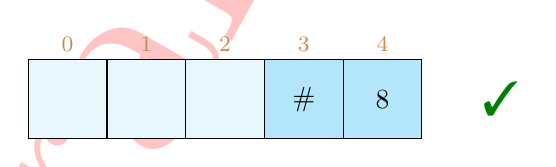
\begin{tikzpicture}
    \filldraw[fill=cyan!10] (0,0) rectangle (1,1);
    \filldraw[fill=cyan!10] (1,0) rectangle (2,1);
    \filldraw[fill=cyan!10] (2,0) rectangle (3,1);
    \filldraw[fill=cyan!30] (3,0) rectangle (4,1) node[midway] {\#};
    \filldraw[fill=cyan!30] (4,0) rectangle (5,1) node[midway] {8};
    \foreach \i in {0,1,2,3,4}
        \node[font=\footnotesize, color=brown!90!] at (\i+0.5, 1.2) {\i};
    \node[font=\LARGE, color=green!50!black] at (6,0.5) {\ding{51}};
  \end{tikzpicture}
\end{figure}

假如把 $h=3$ 位置直接删除,那么查找时,查找 8 的散列位置 $h=3$ 发现是空闲的,就会直接返回「查找失败」,从而产生错误。

\begin{figure}[htb]
  \centering
  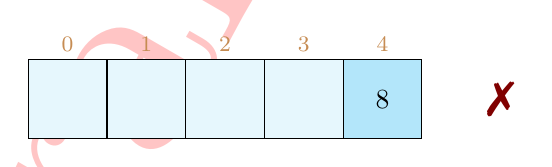
\begin{tikzpicture}
    \filldraw[fill=cyan!10] (0,0) rectangle (1,1);
    \filldraw[fill=cyan!10] (1,0) rectangle (2,1);
    \filldraw[fill=cyan!10] (2,0) rectangle (3,1);
    \filldraw[fill=cyan!10] (3,0) rectangle (4,1);
    \filldraw[fill=cyan!30] (4,0) rectangle (5,1) node[midway] {8};
    \foreach \i in {0,1,2,3,4}
        \node[font=\footnotesize, color=brown!90!] at (\i+0.5, 1.2) {\i};
    \node[font=\LARGE, color=red!50!black] at (6,0.5) {\ding{55}};
  \end{tikzpicture}
\end{figure}

因此,删除散列表的元素时,不能直接删掉,而是应该打标记。

\vspace{2em}

{\color{cyan!80!black} 【结论】C

【点评】本题考察散列表的用法,具体包括元素的插入、删除、查找方式,线性探查再散列的规则,以及平均查找长度(ASL)的计算等。本题的关键在于删除元素时不能直接删掉,而应该打标记,否则就会算出 $ASL=\frac{1+3+2+1+1}{5}=1.4$ 了。据说在考研真题中算是难度比较大的一道题了。
}

\end{document}